\documentclass[hyperref={pdfpagelabels=false}]{beamer}
\usepackage{graphicx}
\usepackage{amsmath,fancybox,color,colordvi,epsfig,verbatim}

\DeclareGraphicsExtensions{.png,.pdf,.jpg}

\usepackage{listings}
\usepackage{ifpdf}
\usepackage{hyperref} % For hyper reference but *essential* for seminar.
\definecolor{redbg}{RGB}{179 27 27} % Red
\definecolor{matemph}{RGB}{102 0 102} % ANL Violet

\hypersetup{pdfpagemode=UseNone,pdfstartview=FitH} % For the initial view.
\hypersetup{colorlinks=true}
\hypersetup{hypertexnames=false} % Eliminates message: pdfTeX warning (ext4)
\hypersetup{urlcolor=red}
\newcommand{\half}{{\textstyle{\frac{1}{2}}}}
\newcommand{\norm}[1]{\left\| #1 \right\|}
\newcommand{\ip}[2]{\left< #1,\;#2 \right>}
\newcommand{\define}{:=}
\newcommand{\function}[3]{#1: #2 \to #3}
\newcommand{\grad}{\mbox{\boldmath $\nabla$}}
\newcommand{\cD} {\mbox{$\cal D$}}
\newcommand{\cY} {\ensuremath{\mathcal{Y}}}
\newcommand{\emp}[1]{\textcolor{matemph}{#1}}
\newcommand{\remp}[1]{\textcolor{redbg}{#1}}
\newcommand{\bremp}[1]{\textcolor{redbg}{\mathbf{#1}}}
\newcommand{\bemp}[1]{\textcolor{matemph}{\mathbf{#1}}}

 \beamertemplatedotitem                 % Dot  symbol in item
 \beamertemplatenumberedsectiontoc      % Number TOC
 \beamersetleftmargin{.5cm}             % Left  margin
 \beamersetrightmargin{.5cm}            % Right margin
 \beamertemplatenavigationsymbolsempty  % No navigation symbols


\usetheme{Malmoe}
\usefonttheme[onlymath]{serif}

%\useframetitletemplate{%
%\vskip0.25em%
%\alert{\Large \insertframetitle}
%\par
%}


\title[Toolkit for Advanced Optimization]{Numerical Optimization and the\\Toolkit for Advanced Optimization}
\author[Jason Sarich]{Jason Sarich, Todd Munson, Jorge Mor\'{e}}
\institute[Argonne National Laboratory]{Mathematics and Computer Science Division, \\Argonne National Laboratory }
\date{August 18, 2010}


%\input{defs}

\begin{document}

\maketitle


\lecture{Numerical Optimization}{Optimization}
\part{Nonlinear Optimization}
\frame{\partpage}
\section{ACTS Workshop 2009}

\frame{
\frametitle{Nonlinear Optimization}
\begin{itemize}
\item{Unconstrained Optimization}
\item{Bound-constrained Optimization}
\item{General Constrained Optimization}
\end{itemize}
}

\frame{
\frametitle{Nonlinear Optimization}
\begin{center}
Unconstrained Optimization Problem
\end{center}
\begin{eqnarray*}
f: \; \mathbb{R}^N \mapsto \mathbb{R} \\
\min_{x \in \mathbb{R}^N}  f(x)  
\end{eqnarray*}
}

\frame{
\frametitle{Nonlinear Optimization}
\begin{center}
Bound-constrained Optimization Problem
\end{center}
\begin{eqnarray*}
\min & f(x) & \mbox{ (objective function) }\\
\mbox{subject to} & x_l \le x \le x_u  & \mbox{ (bounds) }\\
\end{eqnarray*}

}

\frame{
\frametitle{Nonlinear Optimization}
\begin{center}Constrained Optimization Problem\end{center}
\begin{eqnarray*}
\min & f(x) & \mbox{ (objective function) }\\
\mbox{subject to} & c_l \le c(x) \le c_u & \mbox{ (constraints) }\\
\end{eqnarray*}

\textbf{Note}: TAO is not able to solve 
constrained optimization problems directly.

}



\lecture{Algorithms}{Algorithms}
\part{Algorithms}
\frame{\partpage}

\frame{
\frametitle{Algorithms}
Nonlinear optimization algorithms are iterative processes.  
In many cases, each iteration involve calculating a 'search direction', 
then function values along that direction are calculated until
certain conditions are met. 
\begin{itemize}
\item Newton's Method
\item Quasi-Newton Methods
\item Conjugate Gradient
\end{itemize}
}

\frame{
\frametitle{Algorithms}
\begin{center}Newton's Method\end{center}
\begin{itemize}
\item \textcolor{red}{Step 0} Choose initial vector $x_0$
\item \textcolor{red}{Step 1} Compute gradient $\nabla f(x_k)$ and 
Hessian $\nabla^2 f(x_k)$
\item \textcolor{red}{Step 2}
Calculate the direction $d_{k+1}$ by solving the system:
\[
 \nabla^2 f(x_k)  d_{k+1} = - \nabla f(x_k)
\]

\item \textcolor{red}{Step 3} Apply line search algorithm to obtain ``acceptable'' new vector:
\[
 x_{k+1} = x_k + \tau d_{k+1}
\]
\item \textcolor{red}{Return to Step 1}
\end{itemize}
}


\frame{
\frametitle{Algorithms}
\begin{center}Problems with Newton's Method\end{center}
\begin{itemize}
\item Hessian must be derived, computed, and stored
\item Linear solve must be performed on Hessian
\end{itemize}
}

\frame{
\frametitle{Algorithms}
\begin{center}Quasi-Newton Methods \\ 
 Use approximate Hessian $B_k \approx \nabla^2 f(x_k)$.  Choose a formula for $B_k$ so that:
\end{center}
\begin{itemize}
\item $B_k$ relies on first derivative information only
\item $B_k$ can be easily stored
\item $B_{k} d_{k+1} = - \nabla f(x_k)$ can be easily solved
\end{itemize}
}

\frame{
\frametitle{Algorithms}
\begin{center}Conjugate Gradient Algorithms\end{center}
These algorithms are an extension of the conjugate gradient methods for
solving linear systems.
\[
d_{k+1} = - \grad f (x_k) + \beta_k d_k 
\]

\medskip

Some possible choices of $ \beta_k $ ($ g_k = \nabla f (x_k ) $):
 
\[
\beta_k^{FR} = \left (
\frac{\| g_{k+1} \|}{\| g_k \|}
\right ) ^ 2 , \qquad \mbox{Fletcher-Reeves}
\]
\[
\beta_k^{PR} = 
\frac{ \langle g_{k+1} , g_{k+1} - g_k \rangle }
{\| g_k \|^2},  \qquad \mbox{Polak-Ribi\`ere}
\]
\[
\beta_k^{PR+} = \max \left \{ \beta_k^{PR} , 0 \right \} , \qquad
\mbox{PR-plus}
\]
}


\frame{
\frametitle{Algorithms}
\begin{center}Derivate Free Algorithms\end{center}
There are some applications for which it is not feasible to
find the derivative of the objective function.  There are some algorithms
available that can solve these applications, but they can be very slow to
converge.
\begin{itemize}
\item Pattern Searches
\item Nelder-Mead Simplex
\item Model-based methods \remp{Coming soon!}
\item Use finite differences
\end{itemize}
}


\lecture{TAO}{TAO}
\part{TAO}

\frame{\partpage 
The process of nature by which all things change and which is to be
followed for a life of harmony}

\frame{
\frametitle{TAO}
\begin{center}What does TAO do for you?\end{center}
\begin{itemize}
\item Contains a library of optimization solvers for solving unconstrained, bound-constrained, and complementarity optimization problems.  These solvers include Newton methods,
Quasi-Newton methods, conjugate gradients, derivative free, and semi-smooth methods.
\item Provides C, C++, and Fortran interfaces to these libraries
\item Allows for large scale, sparse objects, and parallel applications
\item Uses PETSc data structures and utilities
\end{itemize}
}

\frame{
\frametitle{TAO Solvers}
\begin{tabular}{|c|ccc|}
\hline
     & handles bounds & requires gradient & requires Hessian \\
\hline
lmvm &     no         &      yes          &        no        \\
nls  &     no         &      yes          &       yes        \\
ntr  &     no         &      yes          &       yes        \\
ntl  &     no         &      yes          &       yes        \\
cg   &     no         &      yes          &        no        \\
nm   &     no         &       no          &        no        \\
blmvm&     yes        &      yes          &        no        \\
tron &     yes        &      yes          &       yes        \\
gpcg &     yes        &      yes          &        no        \\
\hline
\end{tabular}
}


\frame{
\frametitle{TAO}
\begin{center} Pressure in a Journal Bearing \end{center}
\[
\min 
\left \{
\int_{ \cD } \left \{ \half  w_q (x) \| \grad v (x) \| ^ 2  -
  w_l (x) v (x) \right \} \, d x : v \ge 0
\right \}
\]
%
\begin{minipage}[b]{.45\linewidth}
\[
\begin{array}{c}
 w_q ( \xi_1 , \xi_2 ) = ( 1 + \epsilon \cos \xi_1 ) ^ 3  \\
 w_l ( \xi_1 , \xi_2 ) = \epsilon \sin \xi_1 \\
 \cD = ( 0 , 2 \pi ) \times ( 0 , 2b ) 
\end{array}
\]
\vspace{0.5em}
\end{minipage} \hfil
\begin{minipage}[b]{.45\linewidth}
\ifpdf
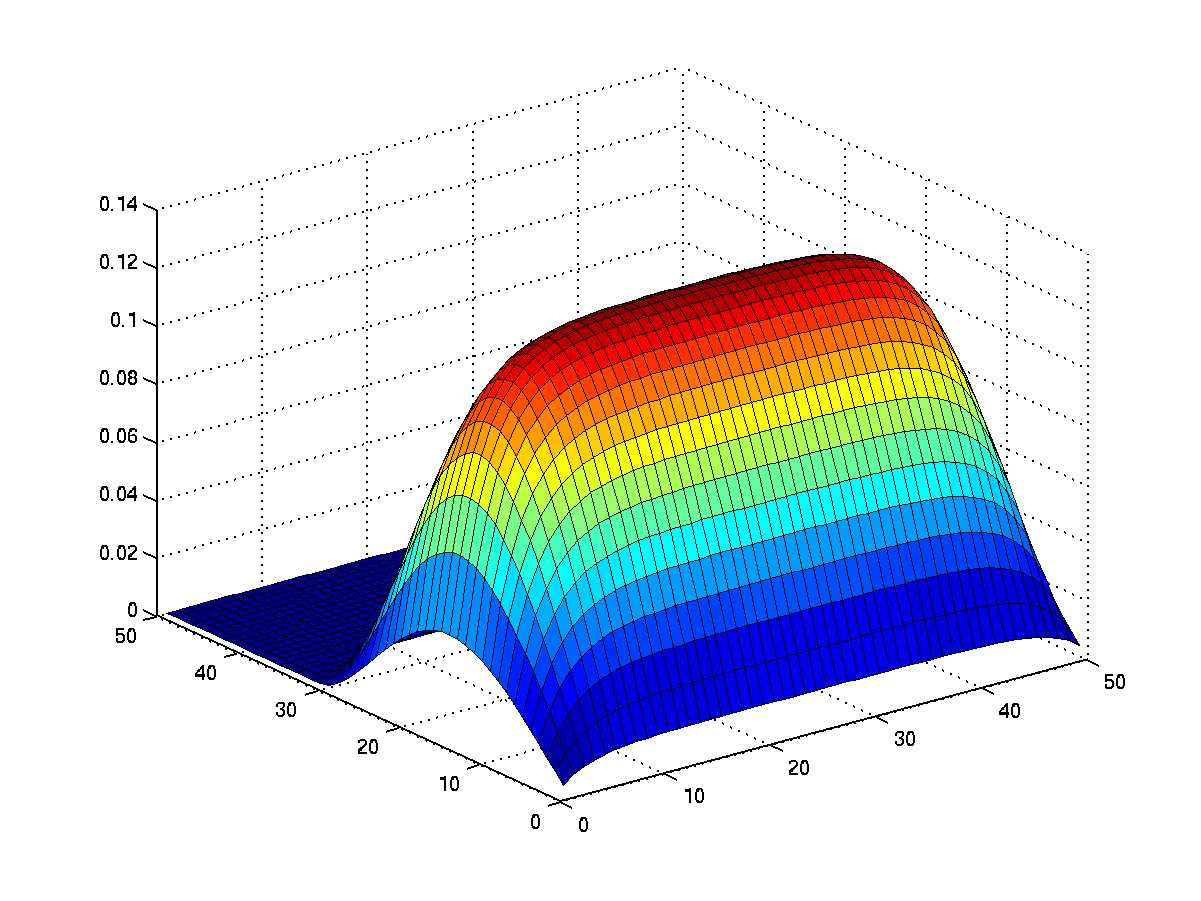
\includegraphics[height=1.2in]{../images/pjb5050}
\else
\fi
\end{minipage}

\medskip

Number of active constraints depends on the choice of 
$ \epsilon $ in $ (0,1) $.  \\
Nearly degenerate problem. Solution $ v \notin C^2 $.

}

\frame{
\frametitle{TAO}
\begin{center}Minimal Surface with Obstacles\end{center}

\[
\min 
\left \{
\int_{ \cD } \sqrt { 1 + \| \grad v (x) \| ^ 2 } \, d x : v \ge v_L
\right \}
\]

\medskip

\begin{center}
\ifpdf
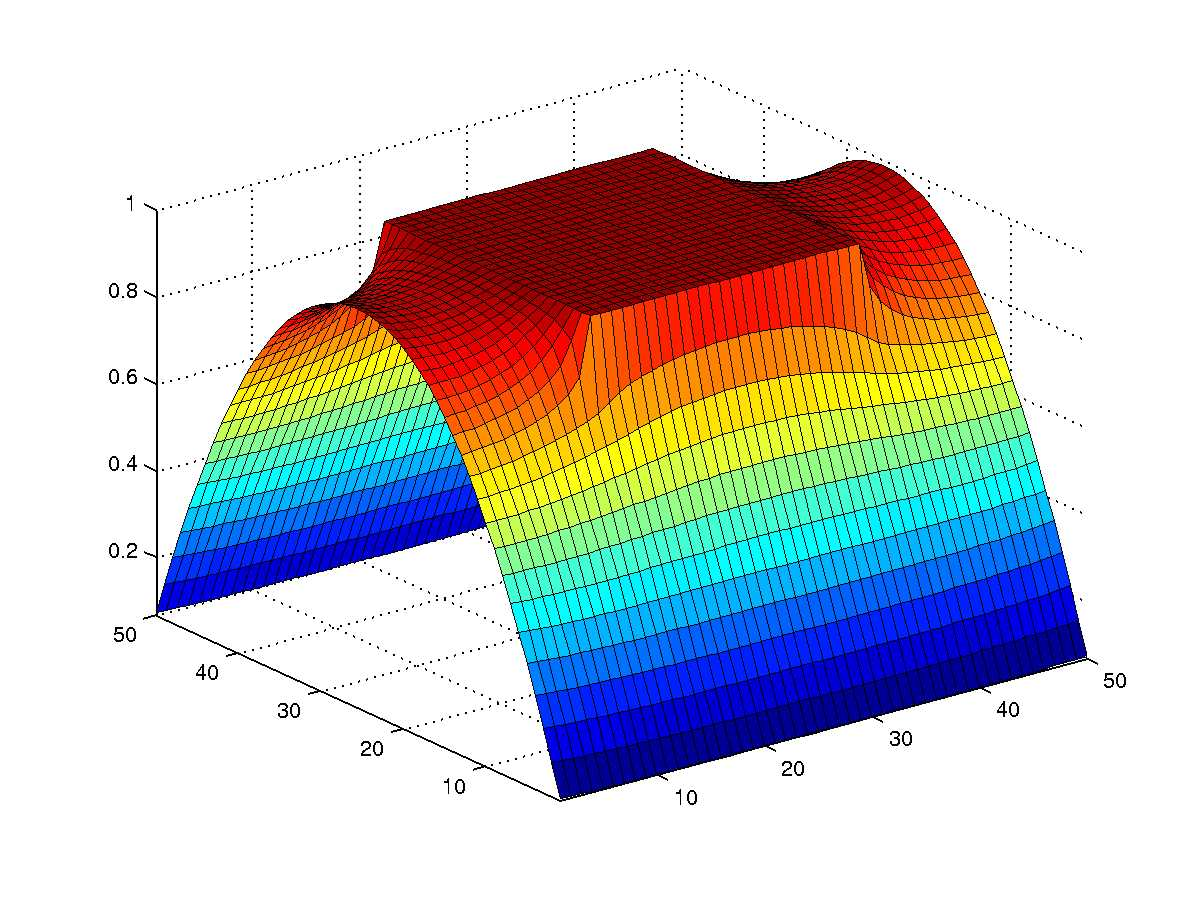
\includegraphics[height=1.2in]{../images/mso_s}
\qquad
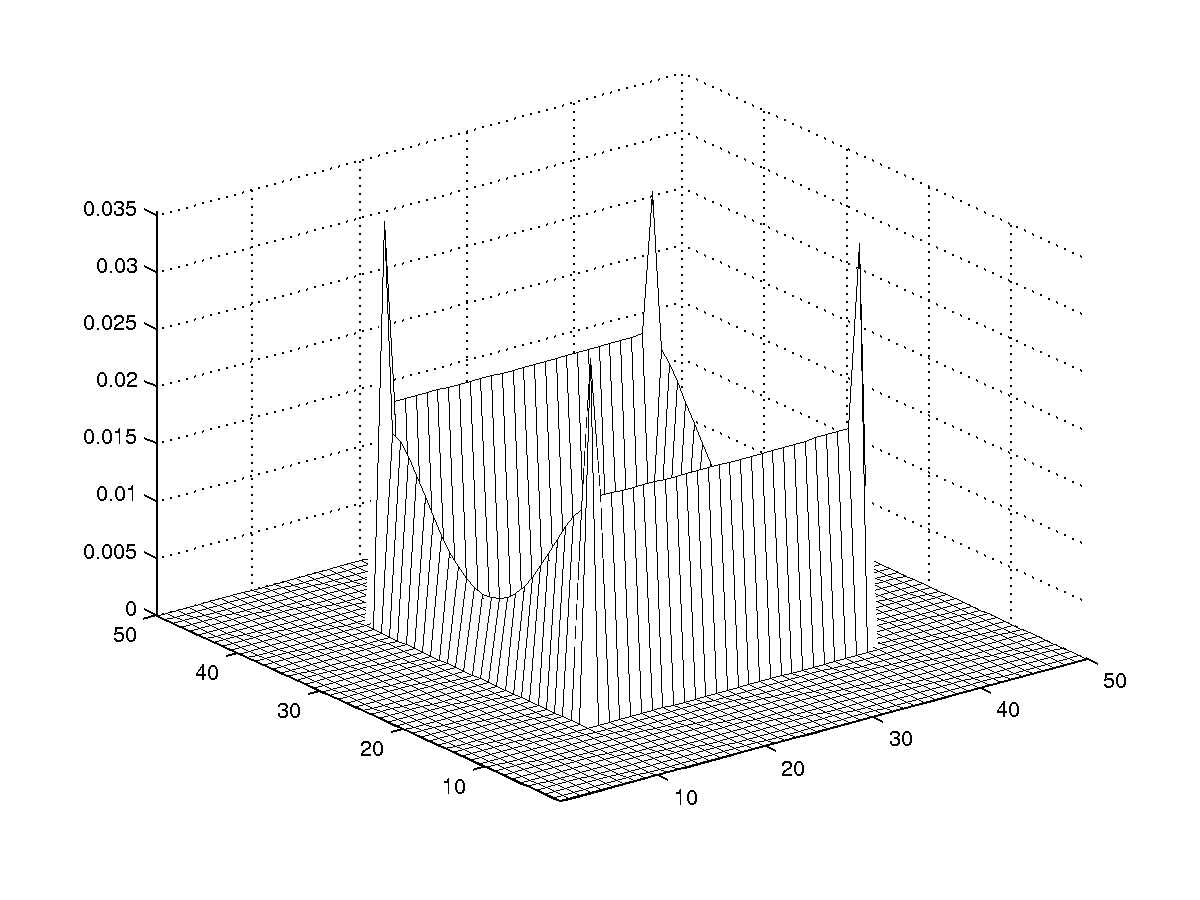
\includegraphics[height=1.2in]{../images/mso_e}
\else
\fi
\end{center}

\bigskip

Number of active constraints depends on the height of the
obstacle. The solution $ v \notin C^1 $.
Almost all multipliers are zero. 

}

\frame{
\frametitle{TAO}
\begin{center}Parallel Performance \end{center}
\begin{table}[bhpt]
\small
\begin{center}
\begin{tabular}{|cccccc|}
\hline
\multicolumn{1}{|c|}{Processors} &
\multicolumn{1}{c|}{BLMVM} &
\multicolumn{1}{c|}{Execution} &
\multicolumn{3}{c|}{Percentage of Time} \\

\multicolumn{1}{|c|}{Used}&
\multicolumn{1}{|c|}{Iterations}&
\multicolumn{1}{c|}{Time}&
\multicolumn{1}{c}{AXPY}&
\multicolumn{1}{c}{Dot} &
\multicolumn{1}{c|}{FG} \\


\hline

8 & 996 & 1083.8 & 31  & 9 & 60 \\ %& 256 \\
16 & 991 & 538.2 & 30 & 10 & 60 \\ %& 580 \\
32 & 966 & 267.7 & 29 & 11 & 60 \\ %& 1137 \\
64 & 993 & 139.5 & 27 & 13 & 60 \\ %& 2027 \\
128 & 987 & 72.4 & 25 & 15 & 60 \\ %& 3728 \\
256 & 996 & 39.2 & 26 & 18 & 56 \\ %& 8009 \\
512 & 1000 & 21.6 & 23 & 22 & 53 \\
\hline
\end{tabular}
\caption{Scalability of BLMVM on Obstacle Problem with 2,560,000 variables. }
\label{routines}
\end{center}
\end{table}

}


\frame{
\frametitle{Mesh Sequencing}
\begin{table}
\begin{center}
%\label{tab:no-mesh}}
\begin{tabular}{|ccc|}
\hline
  Mesh &  niters & Time (s) \\
\hline
 71  $\times$  71   &  6           &   0.58   \\
 141 $\times$  141  &  8           &   1.45   \\
 281 $\times$  281  &  10          &   2.85   \\
 561 $\times$  561  &  21          &   9.34   \\
1121 $\times$  1121 &  $ \dagger $ &    $ \dagger $   \\
2241 $\times$  2241 &  $ \dagger $ &    $ \dagger $   \\
4481 $\times$  4481 &  $ \dagger $ &    $ \dagger $    \\
\hline
\end{tabular}
\end{center}
\end{table}

\tiny
Performance results without mesh sequencing on 140 nodes.
The symbol $ \dagger $ is used if there is no convergence after 100 iterations.

\scriptsize
The results in the table show that the number
of iterations grows as the mesh is refined but that for the
finest meshes we terminate Newton's method after 
$niters = 100 $ iterations. 
Although Newton's method is mesh invariant,
the starting point is assumed to be
in the region of quadratic convergence.
A more careful analysis of these
results, however, shows that the starting point 
is not in the
region of quadratic convergence for any of the grids.

}

\frame{
\frametitle{Mesh Sequencing}

We now consider the use of mesh sequencing.  We start with a
mesh with $ 71 \times 71 $ grid points and, at each
stage, use linear interpolation on the coarse mesh
solution to obtain the starting point for the fine mesh.  
Thus, an $ n_x \times n_y $ coarse mesh becomes
a fine $ (2n_x-1) \times (2n_y-1) $ mesh. We
use the same termination condition 
at each level of refinement.

}

\frame{
\frametitle{Mesh Sequencing}


\begin{table}
\begin{center}
\begin{tabular}{|ccc|}
\hline
  Mesh &  niters & Time (s)  \\
\hline
 71  $\times$  71  &  6     &   0.58    \\
 141 $\times$  141  &  3    &   0.44     \\
 281 $\times$  281  &  2    &   0.52     \\
 561 $\times$  561  &  2    &   1.31     \\
1121 $\times$  1121 &  2    &   5.51     \\
2241 $\times$  2241 &  2    &   19.5     \\
4481 $\times$  4481 &  2    &   189      \\
\hline
\end{tabular}
\end{center}
\end{table}

\tiny
\begin{center}
Performance results with mesh sequencing on 140 nodes.
\end{center}

\scriptsize
The results in this table show 
the performance of the TRON solver on each mesh.
After the solution is obtained on the coarsest
mesh, the number of iterations per mesh is either two or three.
This is the desired behavior for mesh sequencing.
Because the number of Krylov iterations increases on finer meshes,
solution times per level grow at a faster than linear rate.
Better preconditioners may further improve performace.

}


\frame{
\frametitle{POUNDER - Model-based Derivate-free optimization}
\vspace{.15in}
\begin{columns}[t]
\column{.4\paperwidth}
\vspace{.15in}
\begin{figure}[t!]
  \pgfimage[width=\linewidth]{../images/interpmodel}
\end{figure}
\vspace{-.15in}
\centerline{\scriptsize{$n=2$, $|\cY\_k|=4$}}

\column{.5\paperwidth}
using an interpolating quadratic,
\[q_k(x_k+y_i) = f(x_k+y_i), \quad \forall y_i \in \cY_k.\]
\vspace{0.05in}

\begin{itemize}
\item[\remp{$\rightarrow$}] \remp{ Function values are all you have}
\item \emp{ Other models possible}
\item \emp{ Only provide local approximation}
\item \emp{ Coarse models $\leftrightarrow$ smooth noise}
\end{itemize}
\end{columns}
\vfill
}


\frame{\frametitle{POUNDERS - Nonlinear Least Squares}
\footnotesize
\begin{block}{$f(x) = \frac{1}{2} \sum \limits_{i=1}^p (S_i(x)-d_i)^2$}
\begin{itemize}
\item Obtain a vector of output $S_1(x), \ldots, S_p(x)$ with each simulation
\item Approximate:
\vspace{-.1in}
\begin{eqnarray*}
\nabla f(x) &= \sum_i \bremp{\nabla S_i(x)} (S_i(x)-d_i)\\ 
&\rightarrow  \sum_i \bemp{\nabla m_i(x)} (S_i(x)-d_i)
\end{eqnarray*}
\vspace{-.15in}
\begin{eqnarray*}
\nabla^2 f(x) &= \sum_i \bremp{\nabla S_i(x)}\bremp{\nabla S_i(x)}^T + \sum_i(S_i(x)-d_i)\bremp{\nabla^2 S_i(x)} \\
&\rightarrow \sum_i \bemp{\nabla m_i(x)}\bemp{\nabla m_i(x)}^T + \sum_i(S_i(x)-d_i)\bemp{\nabla^2 m_i(x)}
\end{eqnarray*}
\item Model $f$ via Gauss-Newton or similar
\end{itemize} 
\end{block}}


\frame{
\frametitle{POUNDERS for hfbtho}
\begin{columns}
\column{.55\paperwidth}
\vspace{-.7in}
\begin{figure}[t!]
\pgfimage<1>[width=\linewidth]{../images/hfbtho_shootout}
\end{figure}
\column{.38\paperwidth}
  \begin{itemize}
    \item[$\circ$] 72 cores on Jazz
    \item[$\circ$] 12 wall-clock minutes per $f(\mathbf{x})$
    \item[]
    \item POUNDERS: acceptable $\mathbf{x}$ in 3.2 hours
    \item Nelder-Mead: no acceptable $\mathbf{x}$ in 60 hours
  \end{itemize}
\end{columns}
}


\frame{
\frametitle{TAO}
\begin{center}What TAO doesn't do \end{center}
\begin{itemize}
\item{Application Modeling}
\item{Derivatives}
\item{Linear programming}
\item{Constrained optimization}
\item{Integer programming}
\item{Global minimization}
\end{itemize}
}


\frame{
\frametitle{TAO Applications}
\begin{center}Using TAO\end{center}


There are two parts to solving an optimization application with TAO:
\begin{itemize}

\item \textcolor{blue}{An {\bf Application Object} that contain routines to
evaluate an objective function, define constraints on the
variables, and provide derivative information.}

\item \textcolor{green}{A driver program (\texttt{main}) that creates a 
{\bf TAO solver} with desired
algorithmic options and tolerances and connects with the application object.}
\end{itemize}

By default, TAO uses \textcolor{red}{Matrix}, \textcolor{red}{Vector}, and \textcolor{red}{KSP} objects from PETSc but can be extended to other linear algebra packages.

}

\frame{
\frametitle{TAO Application}
%\begin{center}

\centerline {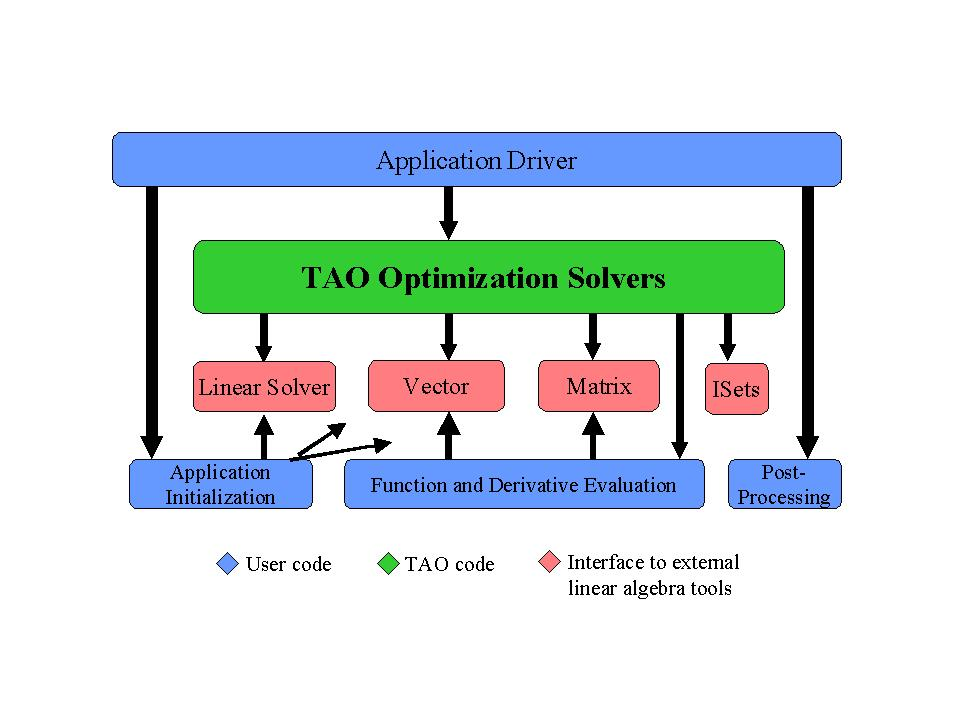
\includegraphics[height=3.5in]{../images/tao_pic3}}


}

\frame{
\frametitle{TAO Applications}
\begin{center}What do you need to do for the \textcolor{blue}{Application Object}?\end{center}
You need to write C, C++, or Fortran functions that:
\begin{itemize}
\item Set the initial variable vector
\item Compute the objective function value at a given vector
\item Compute the gradient at a given vector
\item Compute the Hessian matrix at a given vector (for Newton methods)
\item Set the variable bounds (for bounded optimization)
\end{itemize}
}

\frame[containsverbatim]{
\frametitle{TAO Applications}
Create a data structure that contains any state information,
such as parameter values or data viewers, that the evaluation routines
will need.  For example:
\begin{verbatim}
  typedef struct {          
      double      epsilon; /* application parameter */
      int         n;       /* Size of problem       */
      int         rank;
      int         size;
  } UserContext;
\end{verbatim}
The objective function evaluation routine should look like:
\begin{verbatim}
  int MyFunction(TAO_APPLICATION app, Vec x, 
                       double *fcn, void *userCtx){
     UserContext *user = (UserContext *)userCtx;
     ...
  }

\end{verbatim}
}

\frame[containsverbatim]{
\frametitle{TAO Applications}
The routines for computing the gradient and Hessians look similar:
\begin{verbatim}
  int MyGradient(TAO_APPLICATION app, Vec x, Vec g, 
                       void *userCtx){
     UserContext *user = (UserContext *)userCtx;
     ...
  }
  int MyHessian(TAO_APPLICATION app, Vec x, Mat *H, 
                  Mat *Hpre, int *flag, void *userCtx){
     UserContext *user = (UserContext *)userCtx;
     ...
  }
\end{verbatim}
}

\frame{
\frametitle{TAO Applications}
\begin{center}Writing the Driver\end{center}
A ``driver'' program is used to hook up the user's application to the
TAO library.
This driver performs the following steps:
\begin{itemize}
\item Create the TAO Solver and Application objects
\item Create the variable vector and Hessian matrix
\item Hook up the Application to TAO
\item Solve the application
\end{itemize} 
}

\frame[containsverbatim]{
\frametitle{TAO Applications}
\begin{center}Create the TAO Solver and Application objects\end{center}
\begin{verbatim}
 TAO_SOLVER      tao;  /* TAO Optimization solver     */
 TAO_APPLICATION app;  /* TAO Application using PETSc */
 UserContext     user; /* user-defined structure      */
 Vec             x;    /* solution vector             */
 Mat             H;    /* Hessian Matrix              */

 PetscInitizialize(&argc,&argv,0,0);
 TaoInitialize(&argc,&argv,0,0);
 TaoCreate(PETSC_COMM_SELF,"tao_lmvm",&tao);
 TaoApplicationCreate(PETSC_COMM_SELF,&app);
 ... 
\end{verbatim}
}


\frame[containsverbatim]{
\frametitle{TAO Applications}
\begin{center}Create storage for the solution vector and Hessian 
matrix\end{center}
\begin{verbatim}
 TAO_SOLVER      tao; /* TAO Optimization solver     */
 TAO_APPLICATION app; /* TAO Application using PETSc */
 UserContext     user;/* user-defined structure      */
 Vec             x;   /* solution vector             */
 Mat             H;   /* Hessian Matrix              */

 ...
 VecCreateSeq(PETSC_COMM_SELF,n,&x);
 MatCreateSeqAIJ(PETSC_COMM_SELF,n,n,nz,PETSC_NULL,&H);
 ... 
\end{verbatim}
}


\frame[containsverbatim]{
\frametitle{TAO Applications}
\begin{center}Hook up the application to TAO\end{center}
\begin{verbatim}
 TAO_SOLVER      tao;  /* TAO Optimization solver     */
 TAO_APPLICATION app;  /* TAO Application using PETSc */
 UserContext     user; /* user-defined structure      */
 Vec             x;    /* solution vector             */
 Mat             H;    /* Hessian Matrix              */

 ...
 user.epsilon = 0.1;
 TaoAppSetInitialSolutionVec(app,x);
 TaoAppSetObjectiveRoutine(app,MyFunction,(void *)&user);
 TaoAppSetGradientRoutine(app,MyGradient,(void *)&user);
 TaoAppSetHessianRoutine(app,MyHessian,(void *)&user);
 ... 

\end{verbatim}
}

\frame[containsverbatim]{
\frametitle{TAO Applications}
\begin{center}Solve the application\end{center}
\begin{verbatim}
 TAO_SOLVER      tao;  /* TAO Optimization solver     */
 TAO_APPLICATION app;  /* TAO Application using PETSc */
 UserContext     user; /* user-defined structure      */
 Vec             x;    /* solution vector             */
 Mat             H;    /* Hessian Matrix              */

 ...
 TaoSolveApplication(app, tao);
 VecView(x,PETSC_VIEWER_STDOUT_SELF);
\end{verbatim}
}


\frame[containsverbatim]{
\frametitle{TAO Applications}
\begin{center}Solve a multiple processor application\end{center}
The most important and difficult part of solving a multiple processor
application is writing the function, gradient, and Hessian
evaluation routines to run in parallel. 

Once that is done, it is trivial to get TAO to run in parallel:
\begin{verbatim}
 ...
 TaoCreate(PETSC_COMM_WORLD,"tao_lmvm",&tao);
 TaoApplicationCreate(PETSC_COMM_WORLD,&app);
 VecCreateMPI(PETSC_COMM_WORLD,n,&x);
 MatCreateMPIAIJ(PETSC_COMM_WORLD,n,n,nz,PETSC_NULL,&H);
 ...
\end{verbatim}
}

\frame{
\frametitle{Toolkit for Advanced Optimization}
\begin{itemize}
\item You can download TAO from the webpage \url{http://www.mcs.anl.gov/tao}

\item The documention online includes installation instructions, a user's manual 
and a man page for every TAO function.

\item The download includes several examples for using TAO in C and Fortran.  We
will use some of these examples in the tutorial.

\item If you have any questions, please contact us at \url{tao-comments@mcs.anl.gov}
\end{itemize}
}

\end{document}

